\documentclass{article}

\usepackage{amsmath}
\usepackage{mathtools}
\usepackage{amsfonts}
\usepackage{graphicx}
\usepackage[hidelinks, colorlinks=true, urlcolor=blue, linkcolor=black, citecolor=black]{hyperref}
\usepackage[utf8]{inputenc}
\usepackage[justification=centering]{caption}
\usepackage{geometry}
\usepackage{bm}
\usepackage{array}
\geometry{
	a4paper,
	total={140mm,230mm}
}


\usepackage{xcolor}

% Syntax: \colorboxed[<color model>]{<color specification>}{<math formula>}
\newcommand*{\colorboxed}{}
\def\colorboxed#1#{%
	\colorboxedAux{#1}%
}
\newcommand*{\colorboxedAux}[3]{%
	% #1: optional argument for color model
	% #2: color specification
	% #3: formula
	\begingroup
	\colorlet{cb@saved}{.}%
	\color#1{#2}%
	\boxed{%
		\color{cb@saved}%
		#3%
	}%
	\endgroup
}

\begin{document}
	%	\begin{titlepage}
		%		\begin{center}
			%			\vspace*{-1cm}
			%			\gr
			%			\Huge
			%			\textbf{asdfa}
			%			
			%			\vspace{2cm}
			%			
			%			%\LARGE
			%			\Large
			%			\textbf{asdf}
			%			
			%			\vspace{1cm}
			%			\Large
			%			\textbf{asdfa}
			%			
			%			\textbf{asdfas}
			%			
			%			\vspace{4cm}
			%			
			%			\centering
			%			\makebox[\textwidth][c]{\includegraphics[width=10cm,keepaspectratio]{images/title.png}}
			%			
			%			\vfill
			%			
			%			\vspace{1cm}
			%			\Large
			%			Nikolaos Kotarelas
			%			\vspace{0.25cm}
			%			\\kotarelas@ece.auth.gr
			%			\vspace{0.25cm}
			%			\\January 2023
			%		\end{center}
		%	\end{titlepage}
		
%		\begin{figure}[!htbp]
%			\centering
%			%	\vspace{-0.25cm}
%			\makebox[\textwidth][c]{\includegraphics[width=14cm,keepaspectratio]{../asymptote_resources/point_rotated.png}}
%			\vspace{-0.25cm}
%			\caption{Rotate point $p$ around axis $\hat{\bm{u}}$, by angle $\theta$.}
%		

	\section*{Vehicle-IMU orientation calibration}
	The following method is used to rotate the axii of an IMU arbitrarily placed on a vehicle. The rotation aims in matching the axii of the IMU and the vehicle frame (see picture) in terms of orientation, \textbf{not} in terms of frame origin.
	
	\begin{figure}[!htbp]
		\centering
		%	\vspace{-0.25cm}
		\makebox[\textwidth][c]{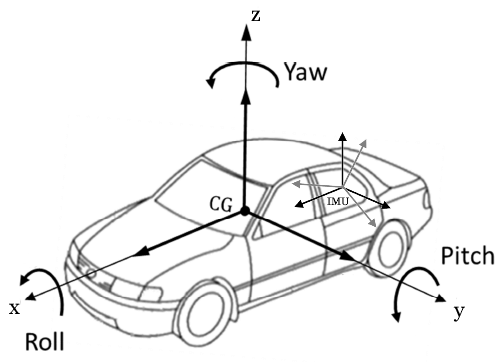
\includegraphics[width=10cm,keepaspectratio]{vehicle_imu_frame.png}}
		\vspace{-0.25cm}
		\caption{Vehicle coordinate frame and IMU coordinate frames. The original IMU orientation (grey) is rotated to match the orientation of the vehicle coordinate frame (black).}
	\end{figure}
	
	The arbitrary orientation of the IMU can be described by rotating the vehicle's coordinate frame around its axii 3 times (one for each axis), as shown below:
	
	\begin{figure}[!htbp]
		\centering
		\vspace{-0.25cm}
		\makebox[\textwidth][c]{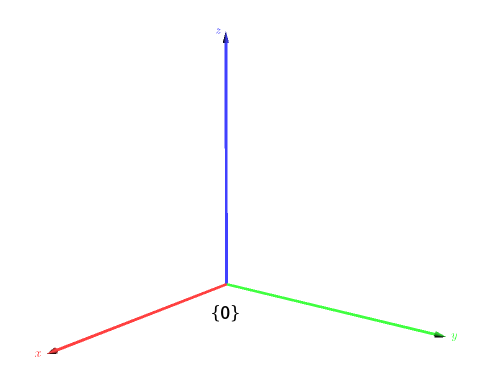
\includegraphics[width=12cm,keepaspectratio]{0_edited.png}}
		\vspace{-1cm}
		\caption{Original vehicle frame orientation.}
	\end{figure}
	
	\newpage
	
	\begin{figure}[!htbp]
		\centering
		\vspace{-0.5cm}
		\makebox[\textwidth][c]{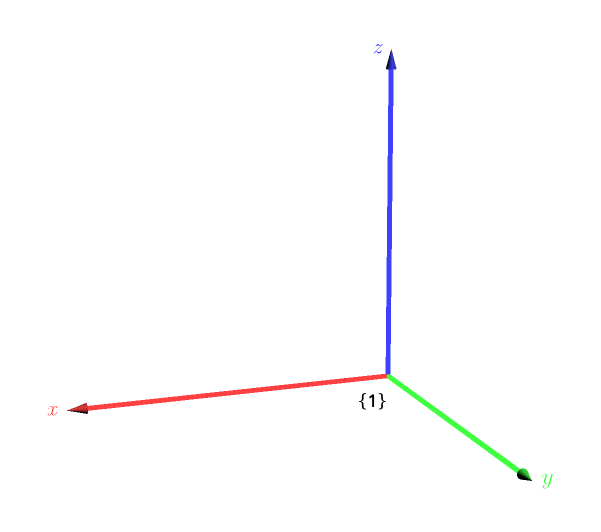
\includegraphics[width=11.5cm,keepaspectratio]{1_edited.png}}
		\vspace{-1.25cm}
		\caption{Result of rotating original vehicle frame around z-axis by -30\textdegree. This frame and the original one share the same z-axis.}
	\end{figure}
	
	\begin{figure}[!htbp]
		\centering
		\vspace{1cm}
		\makebox[\textwidth][c]{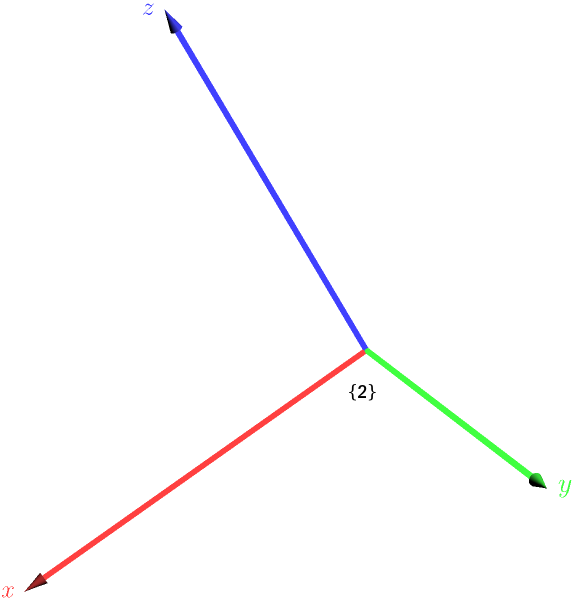
\includegraphics[width=8.6cm,keepaspectratio]{2_edited.png}}
		\vspace{-0.25cm}
		\caption{Result of rotating original vehicle frame around z-axis by -30\textdegree, followed by rotating around y-axis by 30\textdegree.}
	\end{figure}
	
	\newpage
	
	\begin{figure}[!htbp]
		\centering
		\vspace{1cm}
		\makebox[\textwidth][c]{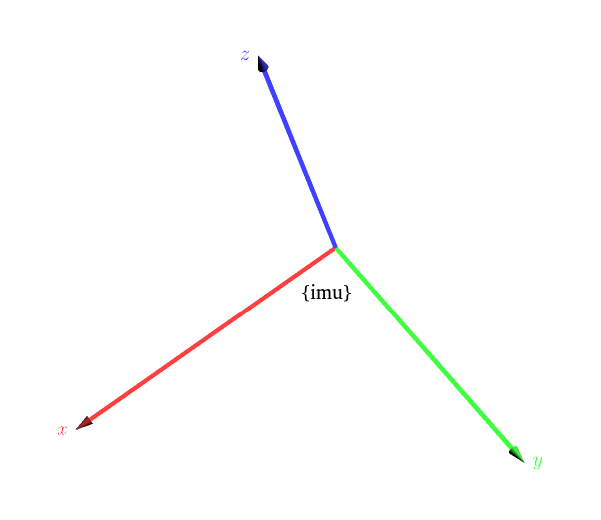
\includegraphics[width=11cm,keepaspectratio]{3_edited.png}}
		\vspace{-0.5cm}
		\caption{Result of rotating original vehicle frame around z-axis by -30\textdegree, followed by rotating around y-axis by 30\textdegree, followed by rotating around x-axis by -30\textdegree.}
	\end{figure}
	
	If we assume the acceleration at each frame is denoted by $\vec{\bm{a}}_{n}$ where $n$ is the name of the frame (see pictures), then the following holds:
	
	\begin{align}
		&\vec{\bm{a}}_{0} = R_z \cdot \vec{\bm{a}}_{1}\label{eqn:c}\\
		&\vec{\bm{a}}_{1} = R_y \cdot \vec{\bm{a}}_{2}\\
		&\vec{\bm{a}}_{2} = R_x \cdot \vec{\bm{a}}_{imu}
	\end{align}
	where:
	\begin{align*}
		&R_z = rodrigues\Big(\begin{bmatrix}0 & 0 & 1\end{bmatrix},\ c\Big)\\
		&R_y = rodrigues\Big(\begin{bmatrix}0 & 1 & 0\end{bmatrix},\ b\Big)\\
		&R_x = rodrigues\Big(\begin{bmatrix}1 & 0 & 0\end{bmatrix},\ a\Big)
	\end{align*}
	
	This means that the acceleration in the calibrated frame $\{0\}$ is connected to the measured acceleration of the IMU through:
	
	\begin{gather}
		\vec{\bm{a}}_{0} = R_z \cdot R_y \cdot R_x \cdot \vec{\bm{a}}_{imu} \\\Leftrightarrow\nonumber\\
		\vec{\bm{a}}_{imu} = R_x^T \cdot R_y^T \cdot R_z^T \cdot \vec{\bm{a}}_{0}
	\end{gather}
	
	Expanding these equations results in:
	\begin{gather}
		\colorboxed{red}{
			\vec{\bm{a}}_{0} = 
			\underbrace{\begin{bmatrix}
				\cos(b) \cos(c) &  \cos(c) \sin(a) \sin(b) - \cos(a) \sin(c) & \sin(a) \sin(c) + \cos(a) \cos(c) \sin(b)\\
				\cos(b) \sin(c) & \cos(a) \cos(c) + \sin(a) \sin(b) \sin(c) & \cos(a) \sin(b) \sin(c) - \cos(c) \sin(a)\\
				-\sin(b) & \cos(b) \sin(a) & \cos(a) \cos(b)
			\end{bmatrix}}_{R_{total}}
			\vec{\bm{a}}_{imu}
		}
	\end{gather}
	
	The point of the calibration is to find the angles $a, b, c$ in order to rotate the measured IMU acceleration $\vec{\bm{a}}_{imu}$ to $\vec{\bm{a}}_{0}$. As it will be explained below, the calibration has to be calculated in two stages.
	
	\section*{Solving for angles}
	\subsection*{Static calibration}
	The first step calculates the angles $a$ and $b$. These have to be calculated when the gravitational vector is constant (does not change orientation, because its norm should be constant). Furthermore, the vehicle must be parallel to the sea level (flat road) and not stand on a slope, otherwise the calculated angles will contain a component related to the slope. These two requirements are satisfied when the vehicle is in a standstill on a flat road, therefore the calibration can be done while vehicle is \textbf{static}.
	
	The result of this first stage matches the z-axis of the two frames, thus rotating the vector $\vec{\bm{a}}_{imu}$ $\rightarrow$ $\vec{\bm{a}}_{1}$ (frame $\{1\}$). The $\vec{\bm{a}}_{1}$ is related to $\vec{\bm{a}}_{imu}$:
	\begin{gather}
		\vec{\bm{a}}_{1} = R_y \cdot R_x \cdot \vec{\bm{a}}_{imu}\Leftrightarrow\nonumber\\
		\colorboxed{red}{
			\vec{\bm{a}}_{1} = 
			\underbrace{\begin{bmatrix}
				\cos(b)  & \sin(a)  \sin(b) &  \cos(a)  \sin(b)\\
				0  		 &          \cos(a) &          -\sin(a)\\
				-\sin(b) &  \cos(b) \sin(a) &  \cos(a)  \cos(b)
			\end{bmatrix}}_{R_{1,imu}}
			\vec{\bm{a}}_{imu}
		}
	\end{gather}
	
	If the vehicle is not in a slope and is not moving, then only the gravitational force is exerted on the IMU sensor. Therefore, the \textit{x} and \textit{y} component of the $\vec{\bm{a}}_{1}$ should be zero. Using the above equation:
	
	\begin{gather}
		a_{1_y} = 0\Leftrightarrow\nonumber\\
		\cos(a) \cdot a_{imu_x} = \sin(a) \cdot a_{imu_z} \label{eqn:a}
	\end{gather}
	and
	\begin{gather}
		a_{1_x} = 0\Leftrightarrow\nonumber\\
		\cos(b) \cdot a_{imu_x} + \sin(a) \sin(b) \cdot a_{imu_y} + \cos(a) \sin(b) \cdot a_{imu_z} = 0\xLeftrightarrow{\cdot \sin(a)} \nonumber\\
		\sin(a) \cos(b) \cdot a_{imu_x} + \sin^2(a) \sin(b) \cdot a_{imu_y} + \cos(a) \sin(b) \underbrace{\sin(a) \cdot a_{imu_z}}_{(\ref{eqn:a})} = 0\Leftrightarrow\nonumber\\
		\sin(a) \cos(b) \cdot a_{imu_x} + \sin(b)\Big( \sin^2(a) \cdot a_{imu_y} + \cos^2(a) \cdot a_{imu_y} \Big) = 0\Leftrightarrow\nonumber\\
		\sin(a) \cos(b) \cdot a_{imu_x} + \sin(b) \cdot a_{imu_y} = 0 \label{eqn:b}
	\end{gather}
	Assuming $a \neq k\dfrac{\pi}{2}$ and $a_{imu_z} \neq 0$, we get using (\ref{eqn:a}):
	\begin{gather}
		\colorboxed{red}{
			a = \arctan2\big(a_{imu_y}, a_{imu_z}\big)
		}
	\end{gather}
	While, assuming $b \neq k\dfrac{\pi}{2}$ and $a_{imu_y} \neq 0$, we get using (\ref{eqn:b}):
	\begin{gather}
		\colorboxed{red}{
			b = \arctan2\big(-\sin(a) \cdot a_{imu_x}, a_{imu_y}\big)
		}
	\end{gather}
	
	\subsection*{Dynamic calibration}
	After rotating $\{imu\}$ frame so its z-axis orientation matches the one with the vehicle's frame ($\{1\}$ frame), we need to calculate the angle $c$ which matches the x and y axii of $\{1\}$ frame to that of the vehicle's frame ($\{0\}$ frame).
	
	In order to proceed with the second stage of the calibration, the angles $a$ and $b$ must have already been found by the first calibration stage. These are necessary since the second stage relies on the $\vec{\bm{a}}_{1}$ vector, as described below.
	
	The acceleration in the vehicle frame ($\vec{\bm{a}}_{0}$) is connected to $\vec{\bm{a}}_{1}$ as seen in (\ref{eqn:c}):
	
	\begin{gather*}
		\vec{\bm{a}}_{0} = R_z \cdot \vec{\bm{a}}_{1} \Leftrightarrow\\
		\vec{\bm{a}}_{0} =
		\begin{bmatrix}
			\cos(c) & -\sin(c) & 0\\
			\sin(c) &  \cos(c) & 0\\
			0 & 0 & 1
		\end{bmatrix}
		\vec{\bm{a}}_{1}
	\end{gather*}
	
	Assuming the vehicle is \textbf{accelerating} in a straight line, the y component of $\vec{\bm{a}}_{0}$ should be zero. This hypothesis gives the solution for angle $c$, assuming $c \neq k\frac{\pi}{2}$ and $a_{1_x} \neq 0$:
	\begin{gather}
		\colorboxed{red}{
			c = \arctan2\big( -a_{1_y}, a_{1_x} \big)
		}
	\end{gather}
	
	\section*{Real-world scenario problems}
	In practice, acceleration readings tend to be noisy. This means that calibration (both static and dynamic) needs to account for errors produced due to the noisy signals. Using only one reading for $\vec{\bm{a}}_{imu}$ should be avoided. Instead, it is encouraged that the conclusion should be drawn from multiple values, spanning a period of time. Some form of low-pass filtering should also prove effective in increasing algorithm robustness. 
	
	When it comes to \textbf{static} calibration, the vehicle, as we described above, is in a standstill. Therefore, the actual acceleration of the vehicle should be constant (only gravity applies). However, due to noise, the readings present with some form of oscillations around the actual acceleration values. We can average out each acceleration axis component to remove the noise and only keep the DC values.
	
	\textbf{Dynamic} calibration on the other hand is more complex. Since the vehicle can not be in a standstill, actual acceleration changes over time through actual physical world phenomena and noise at the same time. We need to clear the noise from the signal, without affecting the effect of these real world phenomena. Therefore, moving average filtering of a time window should be used, designed not to skew the effect of acceleration-changing phenomena. 
	
	Furthermore, we need to detect when these real world phenomena affecting acceleration take place and only use these data for dynamic calibration. Braking seems to be easier to detect than throttling, since commercial vehicles in general have greater braking capabilities than throttling. A threshold method based on the speed provided by the GPS (along with a low-pass filter) should prove effective in detecting braking/throttling events.
	
	
\end{document}